% Vorbereitung: Vorbereitungsaufgaben bearbeiten
% Versuchsaufbau: Verwendete Apparatur, Beschreibung Funktionsweise/Nutzen mit Skizze/Foto
\section{Durchführung}
\label{sec:durchführung}

Im Folgenden werden der Versuchsaufbau zur Bestimmung von Kennlinien einer Hochvakuum-Diode und der Aufbau zur Untersuchung 
des Anlaufstromgebietes beschrieben. Außerdem werden die einzelnen Schritte der Durchführung beider Versuchsteile genannt und erläutert.

\subsection{Kennlinienschar einer Hochvakuum-Diode}
\label{sec:Kennlinieschar}
 
Zunächst wird die Schaltung aus der \autoref{fig:aufbau1} aufgebaut. Darauf wird eine Heizleistung eingestellt.
Diese wird dann noch zwei mal variiert, sodass Messwerte für drei verschiedene Kathodenströme aufgenommen werden.
Für die erste Messung wurde ein Strom von $\SI{2}{\ampere}$ mit einer Spannung von $\SI{3.5}{\volt}$ verwendet.
Bei der zweiten Durchführung wurde ein Strom von $\SI{2.2}{\ampere}$ mit einer Spannung von $\SI{4.5}{\volt}$ angeschlossen.
Beim dritten Mal betrug der Kathodenstrom $\SI{2.4}{\ampere}$ und die Spannung war $\SI{5}{\volt}$ groß.
Die drei Messreihen werden währendessen notiert

\begin{figure}[H]
    \centering
    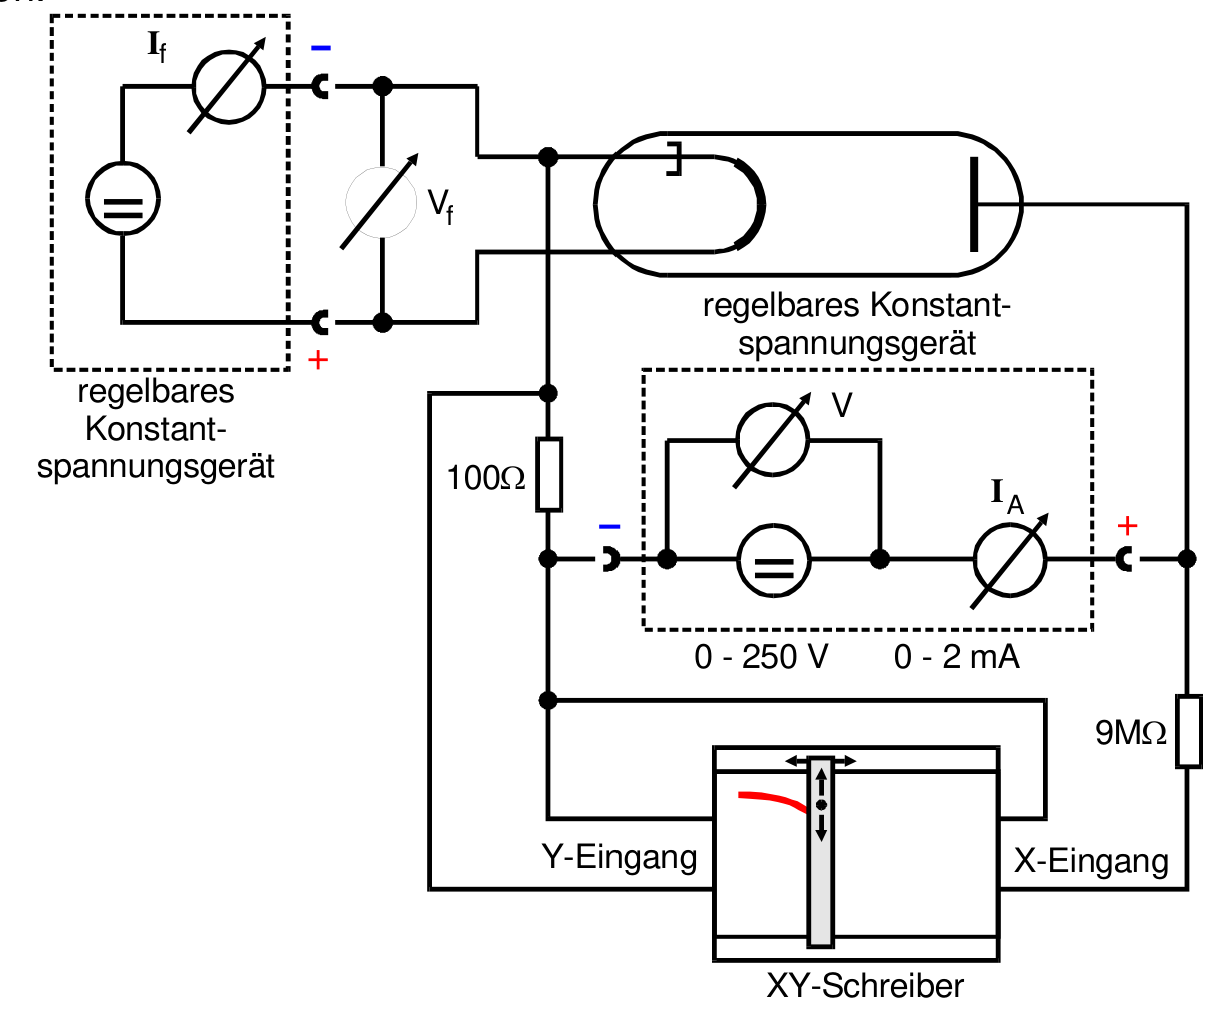
\includegraphics[width=0.5\linewidth]{content/grafik/aufbau1.png}
    \caption{Schaltskizze zur Aufnahme ein Kennlinie eine Hochvakuum-Diode.\cite{elektron}}
    \label{fig:aufbau1}
\end{figure}

\subsection{Untersuchung des Anlaufstromgebietes}
\label{sec:Untersuchung des Anlaufstromgebietes}

Die Schaltskizze aus \autoref{fig:aufbau2} wird aufgebaut.
Es wird eine maximale Heizleistung von $\SI{2.5}{\ampere}$ angeschlossen.
Gemessen wird der Anlaufstrom, während die angeschlossene Spannung von $\SI{0}{\volt}$ bis $\SI{0.9}{\volt}$ includegraphics
0.1-Schritten hochgedreht wird. Die Werte für den Anlaufstrom werden ebenfall notiert.

\begin{figure}[H]
    \centering
    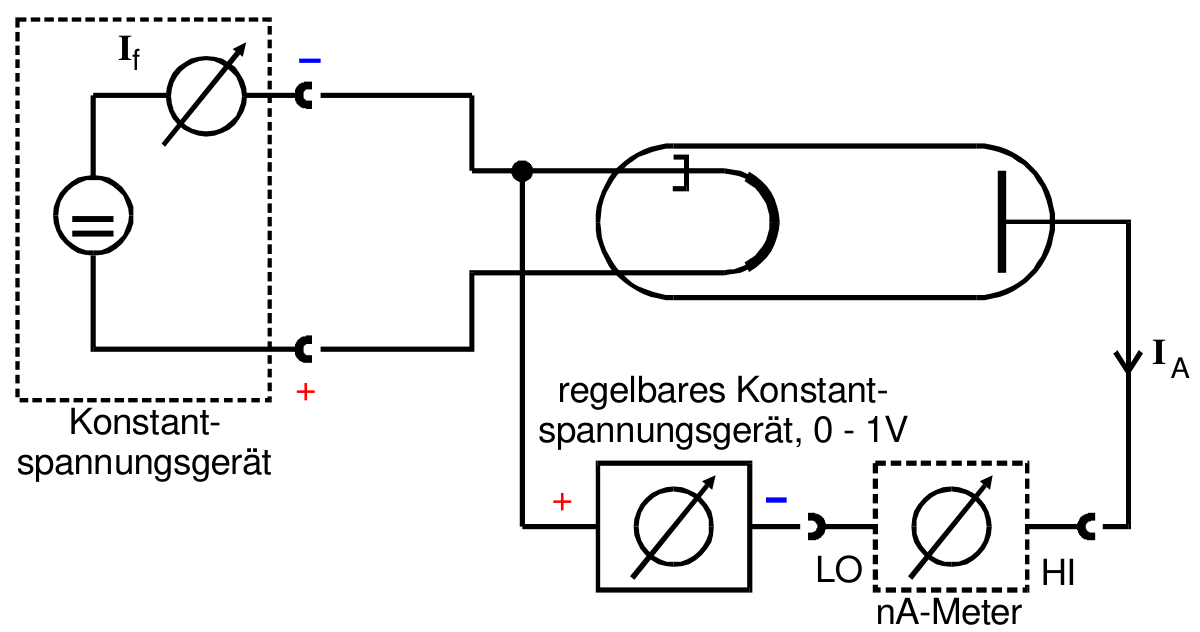
\includegraphics[width=0.5\linewidth]{content/grafik/aufbau2.png}
    \caption{Schaltskizze zur Untersuchung der Anlaufstromgebietes.\cite{elektron}}
    \label{fig:aufbau2}
\end{figure}